\chapter{Implementasi dan Pengujian}
\label{chap:implementasidanpengujian}

Bab ini terdiri atas dua bagian, yaitu Implementasi Perangkat Lunak dan Pengujian Perangkat Lunak. Bagian implementasi berisi penjelasan lingkungan pengembangan perangkat lunak dan hasil implementasi. Sedangkan bagian pengujian berisi hasil pengujian perangkat lunak yang telah dibangun.

\section{Implementasi}
\label{sec:implementasi}

\subsection{Lingkungan Implementasi}
\label{subsec:lingkunganimplementasi}

Implementasi perangkat lunak ini dilakukan di sebuah komputer peneliti untuk keperluan pengujian dan penarikan kesimpulan. Komputer tersebut memiliki spesifikasi sebagai berikut :

\begin{enumerate}
	\item Processor : 1.3GHz
	\item RAM: 4.00 GB DDR3
	\item Sistem Operasi: Windows 10 Home 64-bit
	\item Versi Java : 1.8.0\_92
	\item Koneksi Internet : \textit{bandwidth up to} 1,2MBps
	\item Versi Microsoft Excel : 2016
\end{enumerate}

\subsection{Implementasi Kode Program}
\label{subsec:implementasikodeprogram}

Kode program pada perangkat lunak ditulis dalam bahasa pemrograman Java. Penulisan kode program dibagi menjadi tiga \textit{package} yaitu :\textit{Module}, \textit{Controller} dan \textit{View}. Tujuan penulisan program dibagi menjadi tiga \textit{package} adalah untuk memudahkan proses debuging. Didalam \textit{package Module} merupakan kode-kode program yang menjalankan semua fungsi mulai dari \textit{request} sampai penyimpanan file. Untuk kode program yang ada pada \textit{package Controller} merupakan kode program yang berfungsi untuk menjembatani antara tampilan dengan fungsi-fungsi untuk menjalankan perangkat lunak. Tampilan perangkat lunak ditulis didalam \textit{package View} agar dapat mendukung interaksi antarmuka agar interaksi aplikasi lebih interaktif. Penulisan kode program menggunakan \textit{library} : jsoup dengan versi 1.10.1, JSON dengan versi 20160810 dan swingx-all dengan versi 1.6.4. Untuk kode-kode program tersebut dapat dilihat pada lampiran \ref{chap:kodeprogramA}, lampiran \ref{chap:kodeprogramB} dan lampiran \ref{chap:kodeprogramC}.

\subsection{Tampilan antarmuka}
\label{subsec:tampilanantarmuka}

Berikut ini merupakan hasil implementasi antarmuka untuk perangkat lunak analisis waktu tempuh kota Bandung.
Pada Gambar \ref{fig:implementasiantarmukautama} merupakan tampilan utama dari perangkat lunak yang memiliki tiga buah input yaitu : \textit{radio button}, \textit{datepicker}, \textit{check box}. Terdapat 1 buah tombol \textit{save} yang digunakan untuk melakukan ekstraksi data dan penyimpanan data.

\begin{figure}[H]
				\centering		
				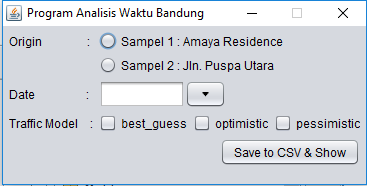
\includegraphics[scale=0.7]{Gambar/gui1.png}
				\caption[Implementasi Antarmuka Utama]{Implementasi Antarmuka Utama}
				\label{fig:implementasiantarmukautama}	
			\end{figure}
			
Pada Gambar \ref{fig:implementasianfilechooser} merupakan tampilan \textit{file chooser} dari perangkat lunak yang memiliki satu buah \textit{window} untuk memilih \textit{directory} penyimpanan file. Terdapat satu buah input untuk memberi nama file. Selain itu tampilan juga terdapat filter file untuk menyimpan data dengan suatu ekstensi tertentu. Terdapat dua buah tombol untuk fitur penyimpanan yaitu : \textit{save} dimana tombol ini berfungsi untuk mengeksekusi penyimpanan file kemudian membuka file tersebut dengan aplikasi Microsoft Excel dan \textit{cancel} untuk membatalkan penyimpanan file.

\begin{figure}[H]
				\centering		
				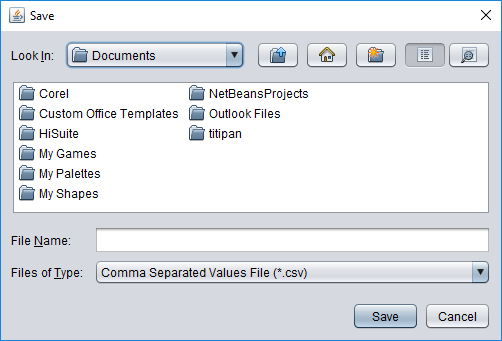
\includegraphics[scale=0.7]{Gambar/gui2.png}
				\caption[Implementasi \textit{file chooser}]{Implementasi \textit{file chooser}}
				\label{fig:implementasifilechooser}	
			\end{figure}
			
\section{Perancangan Pengujian}
\label{sec:perancanganpengujian}

Pengujian perangkat lunak sederhana analisis waktu tempuh kota Bandung dengan memanfaatkan Google Direction API akan berfokus pada hasil ekstraksi data yang dimana data tersebut akan dianalisis dan kesesuaian reaksi perangkat lunak sehingga dapat menjawab dari rumusan masalah yang dipaparkan pada subbab \ref{sec:rumusan}. Pengujian perangkat lunak sederhana ini akan diuji dengan menggunakan \textit{test case} beserta dengan skenarionya. Pengujian ini dilakukan pada lingkungan implementasi sesuai pada subbab \ref{subsec:lingkunganimplementasi}. Terdapat dua tes kasus yang diujikan. Tes tersebut adalah sebagai berikut :
\begin{enumerate}
	\item Pengguna menjalankan program.
	\item Pengguna memasukan input dan menekan tombol save.
\end{enumerate}

\section{Test Case}
\label{sec:testcase}

\textit{Test case} ini dihasilkan dari diagram \textit{use case} yang ada pada subbab \ref{subsec:diagramusecase}. Berikut adalah \textit{test case} beserta skenarionya.

\subsection{Menyimpan data dalam file .csv}
\label{subsec:menyimpandata}

\begin{itemize}
	\item \textit{Basic path} 
	
	User menjalankan perangkat lunak. User memilih salah satu sampel yang akan dihitung. User memilih tanggal untuk dihitung. User memilih semua model \textit{traffic}. User menekan tombol \textit{save}. Perangkat lunak melakukan \textit{request} ke layanan Google Direction sesuai dari masukan yang dipilih oleh user. User memilih \textit{directory} dan memberi nama pada file. User menekan tombol save, kemudian perangkat lunak menampilkan file dengan menggunakan aplikasi Microsoft Excel.
	
	\item \textit{Alternate Path}
	\begin{itemize}
		\item \textit{Alternate Path 1}
		
		User memilih salah satu dari tiga model \textit{traffic}.
		
		\item \textit{Alternate Path 2}
		
		User memilih dua diantara tiga model \textit{traffic}.
		
	\end{itemize}
\end{itemize}

\section{Hasil Pengujian}
\label{sec:hasilpengujian}

\subsection{Hasil Pengujian \textit{Test Case}}
\label{sec:hasilpengujiantestcase}

Pengujian dilakukan pada masing-masing sampel sebanyak 14 kali. Masukan tanggal yang digunakan adalah 8 Mei 2017 dan 15 Mei 2017. Hasil data yang didapat secara detail bisa dilihat pada lampiran \ref{chap:hasilpengujian}. Berikut adalah hasil pengujian dari \textit{test case} yang telah dipaparkan pada subbab \ref{sec:testcase} dan kesesuaian reaksi perangkat lunak :

\begin{longtable}{|p{0.5cm}|p{4cm}|p{4cm}|p{4cm}|}
\centering
No & Aksi Pengguna & Reaksi yang diharapkan & Reaksi Perangkat Lunak \\ \hline
1 & Pengguna menjalankan program & Antarmuka utama ditampilkan & sesuai \\ \hline
2 & Pengguna memasukan input dan menekan tombol save & File berhasil disimpan dan ditampilkan dengan aplikasi microsoft excel & sesuai \\ \hline
 &  & Jika pengguna belum meilih salah satu dari sampel menampilkan pesan "Silahkan pilih sampel yang akan dihitung antara sampel 1 atau sampel 2" & sesuai \\ \hline
 &  & Jika pengguna belum memilih salah satu dari traffic\_model menampilkan pesan "Anda harus memilih minimal salah satu dari 3 traffic model yang telah disediakan" & sesuai \\ \hline
 &  & Jika pengguna belum memilih tanggal menampilkan pesan "Anda belum memilih tanggal, silahkan pilih tanggal" & sesuai \\ \hline
 &  & Jika pengguna memilih tanggal yang sudah lampau atau hari ini menampilkan pesan "Tanggal yang anda masukan adalah masa lampau atau hari ini, silahkan pilihlah tanggal yang akan datang" & sesuai \\ \hline
 &  & Jika pengguna memilih tanggal yang bukan hari senin menampilkan pesan "Tanggal yang anda pilih bukan hari senin, silahkan pilih tanggal yang merupakan hari senin" & sesuai \\ \hline
\caption{Tabel Hasil Pengujian kesesuaian reaksi perangkat lunak}
\label{tab:pengujian1}
\end{longtable}

Pada \ref{tab:pengujian1} dilakukan pengujian sesuai dengan \textit{test case}. Hasil dari pengujian secara detail dijelaskan pada tabel berikut :

\begin{longtable}{|p{0.5cm}|p{2cm}|p{1.3cm}|p{1.3cm}|p{1.5cm}|p{1.8cm}|p{1.8cm}|p{1.8cm}|p{2cm}|}
   no & Nama Skenario & Sampel 1 & Sampel2 & Tanggal & best\_guess & optimistic & pessimistic & hasil \\ \hline
    1 & Menyimpan data dalam file .csv dengan tiga model traffic dipilih & dipilih & ~ & 8 Mei 2017 & dipilih & dipilih & dipilih & file berhasil disimpan dan membuka file dengan menggunakan aplikasi Microsoft Excel \\ \hline
    2 & Menyimpan data dalam file .csv dengan dua model traffic dipilih & dipilih & ~ & 8 Mei 2017 & dipilih & dipilih & ~ & file berhasil disimpan dan membuka file dengan menggunakan aplikasi Microsoft Excel \\ \hline
    3 & Menyimpan data dalam file .csv dengan dua model traffic dipilih & dipilih & ~ & 8 Mei 2017 & dipilih & ~ & dipilih & file berhasil disimpan dan membuka file dengan menggunakan aplikasi Microsoft Excel \\ \hline
    4 & Menyimpan data dalam file .csv dengan dua model traffic dipilih & dipilih & ~ & 8 Mei 2017 & ~ & dipilih & dipilih & file berhasil disimpan dan membuka file dengan menggunakan aplikasi Microsoft Excel \\ \hline
    5 & Menyimpan data dalam file .csv dengan satu model traffic dipilih & dipilih & ~ & 8 Mei 2017 & dipilih & ~ & ~ & file berhasil disimpan dan membuka file dengan menggunakan aplikasi Microsoft Excel \\ \hline
    6 & Menyimpan data dalam file .csv dengan satu model traffic dipilih & dipilih & ~ & 8 Mei 2017 & ~ & dipilih & ~ & file berhasil disimpan dan membuka file dengan menggunakan aplikasi Microsoft Excel \\ \hline
    7 & Menyimpan data dalam file .csv dengan satu model traffic dipilih & dipilih & ~ & 8 Mei 2017 & ~ & ~ & dipilih & file berhasil disimpan dan membuka file dengan menggunakan aplikasi Microsoft Excel \\ \hline
    8 & Menyimpan data dalam file .csv dengan tiga model traffic dipilih & ~ & dipilih & 8 Mei 2017 & dipilih & dipilih & dipilih & file berhasil disimpan dan membuka file dengan menggunakan aplikasi Microsoft Excel \\ \hline
    9 & Menyimpan data dalam file .csv dengan dua model traffic dipilih & ~ & dipilih & 8 Mei 2017 & dipilih & dipilih & ~ & file berhasil disimpan dan membuka file dengan menggunakan aplikasi Microsoft Excel \\ \hline
    10 & Menyimpan data dalam file .csv dengan dua model traffic dipilih & ~ & dipilih & 8 Mei 2017 & dipilih & ~ & dipilih & file berhasil disimpan dan membuka file dengan menggunakan aplikasi Microsoft Excel \\ \hline
    11 & Menyimpan data dalam file .csv dengan dua model traffic dipilih & ~ & dipilih & 8 Mei 2017 & ~ & dipilih & dipilih & file berhasil disimpan dan membuka file dengan menggunakan aplikasi Microsoft Excel \\ \hline
    12 & Menyimpan data dalam file .csv dengan satu model traffic dipilih & ~ & dipilih & 8 Mei 2017 & dipilih & ~ & ~ & file berhasil disimpan dan membuka file dengan menggunakan aplikasi Microsoft Excel \\ \hline
    13 & Menyimpan data dalam file .csv dengan satu model traffic dipilih & ~ & dipilih & 8 Mei 2017 & ~ & dipilih & ~ & file berhasil disimpan dan membuka file dengan menggunakan aplikasi Microsoft Excel \\ \hline
    14 & Menyimpan data dalam file .csv dengan satu model traffic dipilih & ~ & dipilih & 8 Mei 2017 & ~ & ~ & dipilih & file berhasil disimpan dan membuka file dengan menggunakan aplikasi Microsoft Excel \\ \hline
        15 & Menyimpan data dalam file .csv dengan tiga model traffic dipilih & dipilih & ~ & 15 Mei 2017 & dipilih & dipilih & dipilih & file berhasil disimpan dan membuka file dengan menggunakan aplikasi Microsoft Excel \\ \hline
        16 & Menyimpan data dalam file .csv dengan dua model traffic dipilih & dipilih & ~ & 15 Mei 2017 & dipilih & dipilih & ~ & file berhasil disimpan dan membuka file dengan menggunakan aplikasi Microsoft Excel \\ \hline
        17 & Menyimpan data dalam file .csv dengan dua model traffic dipilih & dipilih & ~ & 15 Mei 2017 & dipilih & ~ & dipilih & file berhasil disimpan dan membuka file dengan menggunakan aplikasi Microsoft Excel \\ \hline
        18 & Menyimpan data dalam file .csv dengan dua model traffic dipilih & dipilih & ~ & 15 Mei 2017 & ~ & dipilih & dipilih & file berhasil disimpan dan membuka file dengan menggunakan aplikasi Microsoft Excel \\ \hline
        19 & Menyimpan data dalam file .csv dengan satu model traffic dipilih & dipilih & ~ & 15 Mei 2017 & dipilih & ~ & ~ & file berhasil disimpan dan membuka file dengan menggunakan aplikasi Microsoft Excel \\ \hline
        20 & Menyimpan data dalam file .csv dengan satu model traffic dipilih & dipilih & ~ & 15 Mei 2017 & ~ & dipilih & ~ & file berhasil disimpan dan membuka file dengan menggunakan aplikasi Microsoft Excel \\ \hline
        21 & Menyimpan data dalam file .csv dengan satu model traffic dipilih & dipilih & ~ & 15 Mei 2017 & ~ & ~ & dipilih & file berhasil disimpan dan membuka file dengan menggunakan aplikasi Microsoft Excel \\ \hline
        22 & Menyimpan data dalam file .csv dengan tiga model traffic dipilih & ~ & dipilih & 15 Mei 2017 & dipilih & dipilih & dipilih & file berhasil disimpan dan membuka file dengan menggunakan aplikasi Microsoft Excel \\ \hline
        23 & Menyimpan data dalam file .csv dengan dua model traffic dipilih & ~ & dipilih & 15 Mei 2017 & dipilih & dipilih & ~ & file berhasil disimpan dan membuka file dengan menggunakan aplikasi Microsoft Excel \\ \hline
        24 & Menyimpan data dalam file .csv dengan dua model traffic dipilih & ~ & dipilih & 15 Mei 2017 & dipilih & ~ & dipilih & file berhasil disimpan dan membuka file dengan menggunakan aplikasi Microsoft Excel \\ \hline
        25 & Menyimpan data dalam file .csv dengan dua model traffic dipilih & ~ & dipilih & 15 Mei 2017 & ~ & dipilih & dipilih & file berhasil disimpan dan membuka file dengan menggunakan aplikasi Microsoft Excel \\ \hline
        26 & Menyimpan data dalam file .csv dengan satu model traffic dipilih & ~ & dipilih & 15 Mei 2017 & dipilih & ~ & ~ & file berhasil disimpan dan membuka file dengan menggunakan aplikasi Microsoft Excel \\ \hline
        27 & Menyimpan data dalam file .csv dengan satu model traffic dipilih & ~ & dipilih & 15 Mei 2017 & ~ & dipilih & ~ & file berhasil disimpan dan membuka file dengan menggunakan aplikasi Microsoft Excel \\ \hline
        28 & Menyimpan data dalam file .csv dengan satu model traffic dipilih & ~ & dipilih & 15 Mei 2017 & ~ & ~ & dipilih & file berhasil disimpan dan membuka file dengan menggunakan aplikasi Microsoft Excel \\ \hline
	\caption {Tabel Hasil Pengujian \textit{test case} perangkat lunak}
		\label{tab:pengujian2}
		\end{longtable}%